\documentclass[twocolumn,english]{IEEEtran}
\usepackage[T1]{fontenc}
\usepackage{babel}
\usepackage{amsthm}
\usepackage{amsmath}
\usepackage{graphicx}
\usepackage[unicode=true,
 bookmarks=true,bookmarksnumbered=true,bookmarksopen=true,bookmarksopenlevel=1,
 breaklinks=false,pdfborder={0 0 0},backref=false,colorlinks=false]
 {hyperref}
\usepackage{bm}
\usepackage{amsmath}
\usepackage{amssymb}
\usepackage{array}
\usepackage{calc}
\usepackage{booktabs}
\newcolumntype{W}{>{\centering\arraybackslash}m{25mm}}
\newcolumntype{L}{>{\centering\arraybackslash}m{15mm}}



\hypersetup{
 pdftitle=  {Lab 5: RC Circuits},
 pdfauthor= {Adam Olson, Nick Lonsdale, Zack Garza},
 pdfpagelayout=OneColumn, pdfnewwindow=true, pdfstartview=XYZ, plainpages=false}

\makeatletter


%%%%%%%%%%%%%%%%%%%%%%%%%%%%%% Textclass specific LaTeX commands.
 % protect \markboth against an old bug reintroduced in babel >= 3.8g
 \let\oldforeign@language\foreign@language
 \DeclareRobustCommand{\foreign@language}[1]{%
   \lowercase{\oldforeign@language{#1}}}
\theoremstyle{plain}
\newtheorem{thm}{\protect\theoremname}
\theoremstyle{plain}
\newtheorem{lem}[thm]{\protect\lemmaname}

%%%%%%%%%%%%%%%%%%%%%%%%%%%%%% User specified LaTeX commands.
% for subfigures/subtables
\ifCLASSOPTIONcompsoc
\usepackage[caption=false,font=normalsize,labelfont=sf,textfont=sf]{subfig}
\else
\usepackage[caption=false,font=footnotesize]{subfig}
\fi

\makeatother
\providecommand{\lemmaname}{Lemma}
\providecommand{\theoremname}{Theorem}
\setcounter{topnumber}{2}
\setcounter{bottomnumber}{2}
\setcounter{totalnumber}{4}
\renewcommand{\topfraction}{0.85}
\renewcommand{\bottomfraction}{0.85}
\renewcommand{\textfraction}{0.15}
\renewcommand{\floatpagefraction}{0.7}
\usepackage{float}
\begin{document}
\onecolumn
\title{Lab 5: RC Circuits}


\author{Adam Olson, Nick Lonsdale, Zack Garza}


\IEEEspecialpapernotice
{Engineering 17L \\
Effective Date of Report: April 22, 2014}


\markboth{Lab 5: RC Circuits}{Zack Garza}
\maketitle
\thispagestyle{plain}
\pagestyle{plain}

\begin{abstract}
The purpose of this lab is to explore some common applications of RC Circuits -- in particular, circuits that effectively perform mathematical operations and circuits that selectively filter input signal frequencies.
\end{abstract}

\tableofcontents

\twocolumn

\listoffigures

\hrulefill


\section{Introduction}
\IEEEPARstart{T}{he}purpose of this experiment is to explore the various functions of the differentiator, integrator, high-
pass, low-pass, and band-pass circuits. Through the data taken we will be able to discern the general

function and possible applications of these circuits. Our analysis will begin with the theory behind said

circuits, we will then use the listed equipment to carry out the procedure which will lead us to our

results which will in turn be followed by our conclusions.

\section{Theory}
	\subsection{Differentiator}

	\begin{figure}[H]
			\begin{centering}
			\begin{center}
			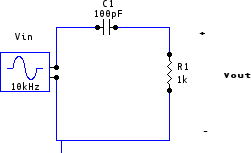
\includegraphics[width=.85\linewidth]{./Circuits/Differentiator.png}
			\caption{Differentiator Circuit Diagram}
			\label{diag:differentiator}
			\end{center}
			\par\end{centering}
	\end{figure}
	The differentiator circuit shown above is a simple high-pass filter.
	This circuit is called a differentiator because the voltage across the resistor actually represents the derivative of the input function.
	Given that the circuit above is a basic passive differentiator, we should be able to observe the differentiator in action within certain frequencies.\cite{wiki-differentiator}


	\subsection{Integrator}
	\begin{figure}[H]
			\begin{centering}
			\begin{center}
			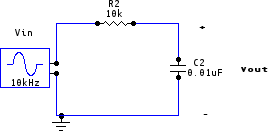
\includegraphics[width=.85\linewidth]{./Circuits/Integrator.png}
			\caption{Integrator Circuit Diagram}
			\label{diag:integrator}
			\end{center}
			\par\end{centering}
	\end{figure}
	This integrator circuit is the most basic version of a low pass filter but is also called an integrator because the voltage across the capacitor is actually the integral of the input function.
	Since this is a basic passive integrator, we should be able to observe the fundamental function of the circuit within certain parameters, i.e., at certain frequencies the effects may break down.\cite{wiki-integrator}

	\subsection{Low-Pass Filter}
	\begin{figure}[H]
			\begin{centering}
			\begin{center}
			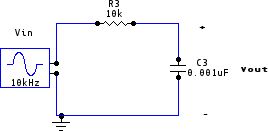
\includegraphics[width=.85\linewidth]{./Circuits/LowPassFilter.png}
			\caption{Low-Pass Filter Circuit Diagram}
			\label{diag:lowpass}
			\end{center}
			\par\end{centering}
	\end{figure}
	The circuit shown here is a passive low pass filter.
	As the name suggests, a low pass filter removes high frequencies and allows only frequencies below a certain point to pass.
	The frequency at which the filter engages is called the cut-off frequency, the cut-off frequency for this particular circuit is $5,915Hz$, meaning all frequencies higher than this frequency should be cut out.
	We expect to see a decrease in amplitude, a phase shift, and a cut-off point in our output function as we scan over various frequencies.
	\begin{align}
		\omega_c = \frac{1}{2\pi RC} = \frac{1}{2\pi (10 k\Omega)(.001 \mu F)} \\
		\Rightarrow \omega_c = 15,915 Hz \notag
	\end{align}

	\subsection{High-Pass Filter}
	\begin{figure}[H]
			\begin{centering}
			\begin{center}
			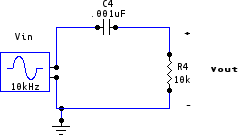
\includegraphics[width=.85\linewidth]{./Circuits/HighPassFilter.png}
			\caption{High-Pass Filter Circuit Diagram}
			\label{diag:highpass}
			\end{center}
			\par\end{centering}
	\end{figure}
	The circuit shown above is a high-pass filter.
	The function of a high-pass filter is to screen out the lower frequencies and only allow the high frequencies to reach the source.
	As with the low-pass filter there is a cut-off frequency for this circuit.
	The cut-off frequency for this particular circuit is $15,915 Hz$, just as with the low pass filter.
	This means that any frequency below the cut-off will not come through.
	\begin{align}
		\omega_c = \frac{1}{2\pi RC} = \frac{1}{2\pi (10 k\Omega)(.001 \mu F)} \\
		\Rightarrow \omega_c = 15,915 Hz \notag
	\end{align}

	The differentiator from Part 1 resembles the low-pass filter from Part 3, and similarly the integrator from Part 2 resembles the high-pass filter.
	This correlation is significant because it shows that in an RC circuit the voltage across the capacitor is the derivative of the source function, just as the voltage across the resistor is the integral of the source function.

	Some applications of the circuits explored in this lab can be seen in audio equipment. The high pass filter is often used to boost the performance of mid-range or tweeter speakers as it blocks out the lower frequencies associated with bass and only allows mid and treble signals to reach the speaker, modeled here by our resistor.
	Inversely, a low pass filter would be used to improve the sound quality of a sub woofer by filtering out high frequencies and passing on the low frequencies so your woofer has that deep boom boom boom.

	Both of these circuits can of course be tweaked to send each respective speaker its optimal signal.
	This can be accomplished by simply using the given impedance of the speaker and the desired frequency, then solving for the proper capacitor.
	If you were really trying to be specific, maybe for a mid-range speaker, you could use a band-pass filter to cut out the highs and the lows, or include just a little high and a little low. We will look at the band-pass filter in Part 5.

	\subsection{Band-Pass Filter}
	\begin{figure}[H]
			\begin{centering}
			\begin{center}
			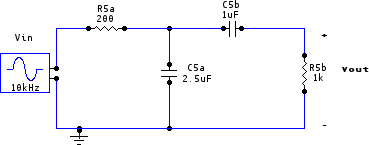
\includegraphics[width=\linewidth]{./Circuits/BandPassFilter.png}
			\caption{Band-Pass Filter Circuit Diagram}
			\label{diag:bandpass}
			\end{center}
			\par\end{centering}
	\end{figure}
	A band-pass filter functions like a combination of the low-pass and high-pass filters, and serves to attenuate all frequencies that are outside of a specific range of frequencies. This effectively restricts the output to a specific ``passband'' of permitted frequencies. Such filters can be used on a signal to reduce or eliminate noise, or to remove unneeded frequencies as a means of compression. They also find common applications in wireless devices and bandwidth limiters, and serve to reduce interference and noise between competing signals.

\hrulefill

\section{Equipment List}
	\begin{enumerate}
		\item Function Generator
		\item Digital Oscilloscope (2 Channel)
		\item Breadboard
		\item Resistors;
			\begin{enumerate}
				\item 1x 1.0 k$\Omega$, ($\frac{1}{4}$W)
				\item 2x 10.0 k$\Omega$, ($\frac{1}{4}$W)
			\end{enumerate}
		\item Capacitors
			\begin{enumerate}
				\item 1x .01 $\mu$F
				\item 1x 100 pF
				\item 2x .001 $\mu$F
			\end{enumerate}
	\end{enumerate}

\hrulefill

\section{Methodology}
	\subsection{Differentiator}
	\begin{enumerate}
		\item Components from equipment list were gathered, and resistance/capacitance values were measured with a DMM.
		\item Breadboard was tested with DMM for any breaks.
		\item Connected a 100 pF capacitor in series with a 1k$\Omega$ resistor on a protoboard as shown in Figure~\ref{diag:differentiator}.
		\item Used a function generator to produce an 10kHz input signal to act as the power source for the Differentiator circuit shown in Figure~\ref{diag:differentiator}.
		\item Measured the voltage across the 1k$\Omega$ resistor  (which was in series with the 100 pF capacitor) using an oscilloscope.
		\item Varied the input signal to generate triangle, square, and sine waves in order to analyze the circuit's response.
		\item Varied the frequency, amplitude, and DC offset of the input signal. Recorded results and captured oscilloscope output.
	\end{enumerate}

	\subsection{Integrator}
	\begin{enumerate}
		\item Connected a 10k$\Omega$ resistor in series with a 0.01$\mu$F capacitor on a protoboard as shown in Figure~\ref{diag:integrator}.
		\item Used as 10kHz input signal at maximum amplitude to drive the Integrator circuit shown in Figure~\ref{diag:integrator}.
		\item Measured the voltage across the 0.01$\mu$F capacitor (which was in series with the 10k$\Omega$ resistor) using the oscilloscope.
		\item Varied the input signal between triangle, square, and sine waves to aid in analyzing the circuit's response.
		\item Varied the frequency, amplitude, and DC offset of the signal, as well as the DC/AC coupling of the oscilloscope. Recorded results and captured scope output.
	\end{enumerate}

	\subsection{Low-Pass Filter}
	\begin{enumerate}
		\item A 10k$\Omega$ resistor was wired in series with a .001$\mu$F capacitor on the protoboard as shown in Figure~\ref{diag:lowpass}.
		\item The oscilloscope and a DMM were wired to measure the voltage across the resistor ($V_{in}$) and the voltage across the capacitor ($V_{out}$) respectively.
		\item The generator was configured to produce a sine wave at a low frequency.
		\item The range of frequencies produced by the generator was swept from the order of 10 kHz to the order of 1 MHz, and measurements were systematically taken for $V_{in}$ and $V_{out}$.
		\item The critical frequency was determined at which the circuit transitioned from ``passing'' to not ``passing'' frequencies.
	\end{enumerate}

	\subsection{High-Pass Filter}
	\begin{enumerate}
		\item A 0.001$\mu$F capacitor was wired in series with a 10k$\Omega$ resistor on a protoboard as shown in Figure~\ref{diag:highpass}.
		\item The scope and DMM were wired to measure the voltage across the capacitor ($V_{in}$) and the voltage across the resistor ($V_{out}$).
		\item A sine wave was used as the input signal, and the range of generator frequencies was again swept from the 10 kHz range to the 1 MHz range.
		\item Input and output voltages were recorded in order to determine the critical frequency of the circuit.
	\end{enumerate}

	\subsection{Band-Pass Filter}
	\begin{enumerate}
		\item A theoretical model of the circuit shown in Figure~\ref{diag:bandpass} was assembled in Circuit Maker, and theoretical values were obtained for the frequencies passed.
		\item The circuit was constructed on a protoboard, and the cutoff frequencies were approximated and measured.
	\end{enumerate}


\hrulefill

\section{Results}

Since the circuits used are all variations of series RC circuits, the expression for cutoff frequency $\omega_c$ is identical for each circuit, and is given by
\begin{equation}
	\omega_c = \frac{1}{RC}.
\end{equation}

From this expression a theoretical cutoff frequency can be calculated for each circuit, as well as a measured cutoff frequency from the measured values of resistance and capacitance in each circuit. This is summarized in Table~\ref{tb:measured_values}.

%%%%%%%%%%%%%%%%%% Measured Data %%%%%%%%%%%%%%%%%%%%%%%%%%%%%%%%
\begin{table}[H]
	\caption{Measured Values of Circuit Elements Used}
	\label{tb:measured_values}
	\begin{tabular}{@{}lllll@{}}

	\toprule
	\textbf{Element}		& \textbf{Differentiator} 	& \textbf{Integrator} 	& \textbf{Low-Pass Filter} 	& \textbf{High-Pass Filter}	\\ \midrule
	{Capacitor}				& 108.6 pF					& 7.6 nF             	& 1.180 nF        			& 1.315 nF           		\\
	{Resistor} 				& 0.989 k$\Omega$ 			& 9.76 k$\Omega$ 		& 9.80 k$\Omega$			& 9.80 k$\Omega$            \\ \midrule
	$\omega_c$ \\(Measured)		& N/A						& N/A					& 86.5 kHz					& 77.6 kHz					\\
	$\omega_c$\\ (Theoretical)	& N/A						& N/A					& 100 kHz					& 100 kHz					\\
	\bottomrule
	\end{tabular}
%%%%%%%%%%%%%%%%%%%%%%%%%%%%%%%%%%%%%%%%%%%%%%%%%%%%%%%%%%%%%%%%%%

\end{table}

	\subsection{Differentiator}
	The output of the differentiator circuit was indeed a good approximation of the derivative of the input signal, and its behavior is summarized in the Figures on Page~\pageref{fig:d1}. The output mirrors any changes in the input, such as adding a DC offset or increasing the amplitude, however changing the frequency causes drastic changes. The figures on the next page show the behavior of three types of waves at a relatively high constant frequency, as well as a single wave at a low frequency.

	When driven by a sine wave (Figure~\ref{fig:d1}) the output is also sinusoidal -- however, it exhibits a noticeable phase shift. Ideally, it would be expected that the phase shift would be $\pi$ radians, or in other words, that the output would resemble a cosine function, but increasing the resolution to the nanosecond scale showed that it was not a perfect derivative.

	Similarly, a square wave examined at the nanosecond scale (Figure~\ref{fig:d2}) showed that neither the voltage nor the output was actually a discrete square wave, but was rather a rough approximation. However, the output was still a good representation of the slope of the original function.

	The output of a triangle wave (Figure~\ref{fig:d3}) appeared to be a square wave at first approximation, but increasing the resolution revealed how the behavior of the capacitor affected this approximation. The output signal was in fact continuous at all points, including points where the derivative would theoretically be undefined, and exhibited the exponential growth/decay pattern characteristic of a capacitor charging and discharging.\\ \\
	Figure~\ref{fig:d4} demonstrates the intended behavior of the circuit, which became apparent at the microsecond scale at low frequencies. The output approximated the derivative of a constant (i.e., zero) at all points, with sharp spikes at the points where the signal changes abruptly.

\clearpage

\begin{figure}[H]
	\centering
	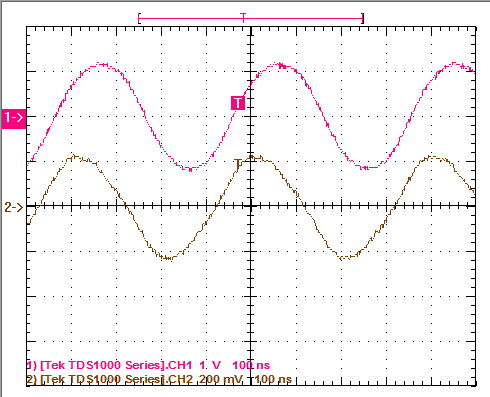
\includegraphics[width=.95\linewidth]{{./Captures/circuit_1_sine_wave_2.5MHz}.png}
	\caption{Differentiator Output Driven by a High Frequency Sine Wave}
	\label{fig:d1}
\end{figure}
The first three input signals were driven at 2.5 MHz and examined on the 100 ns scale. Here, the top signal is the input, and the bottom is the output. The function approximates the derivative of the sine function -- but not perfectly. Note that the differentiator scales down the magnitude of the output signal on the order of $10^{-3}$ volts, and introduces a small phase lag instead of a full $90^{\circ}$ shift.

\vfill

\begin{figure}[H]
	\centering
	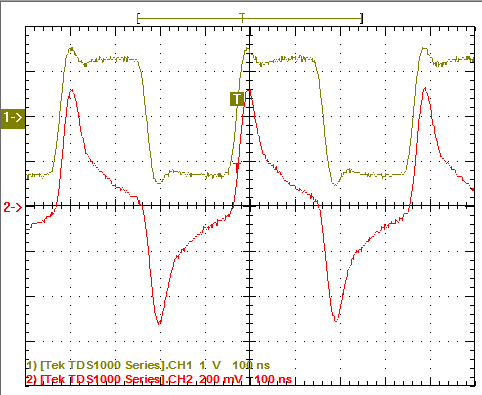
\includegraphics[width=.95\linewidth]{{./Captures/circuit_1_squarewave_2.5Mhz}.PNG}
	\caption{Differentiator Output Driven by a High Frequency Square Wave}
	\label{fig:d2}
\end{figure}
Here, the input (a square wave) is again shown on top, and its output below, and the driving frequency was again 2.5 MHz. On the 100 ns scale, the band-limited behavior of the generator is shown as the square wave is approximated by the sum of sinusoids. Despite this fact, the differentiator still functions as expected, where the output is negative when the input is decreasing and vice-versa.

\break

\begin{figure}[H]
	\centering
	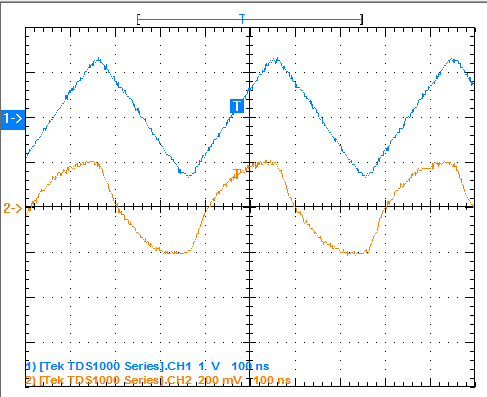
\includegraphics[width=.95\linewidth]{{./Captures/circuit_1_trianglewave_2.5MHz}.PNG}
	\caption{Differentiator Output Driven by a High Frequency Triangle Wave}
	\label{fig:d4}
\end{figure}
The final input at 2.5 MHz was a triangle wave, which is again shown on top. The derivative of a triangle wave would be expected to be a square wave, with constant positive values on the rising edge and constant negative values on the falling edge. This demonstrates the physical limitations of the RC circuit's ability to differentiate, as it takes a small but nonzero amount of time for the capacitor to switch the sign of its voltage.

\vfill

\begin{figure}[H]
	\centering
	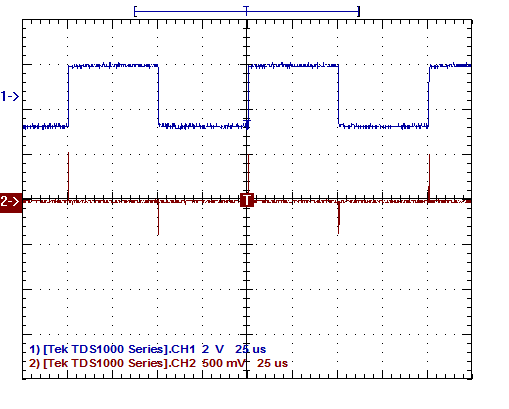
\includegraphics[width=.95\linewidth]{{./Captures/circuit_1_squarewave_10khz}.PNG}
	\caption{Differentiator Output, Driven by a Low Frequency Square Wave}
	\label{fig:d3}
\end{figure}
A square wave driven at 10 kHz and examined at the 25 $\mu$s provides a good first approximation of the derivative of a constant function, as the output is zero nearly everywhere. Since the square wave is a continuous instead of a discrete, piece-wise function, the value of $\frac{dV}{dt}$ is simply instead of undefined. This leads to the large positive and negative spikes in the output when the input voltage switches.


\clearpage

	\subsection{Integrator}

	The integrator circuit behaves similarly to the differentiator circuit, which is summarized in the figures on page~\pageref{fig:i1}. This circuit also produced a signal that varied directly with the input signal. Changes in the amplitude and DC offset were similarly mirrored in the output, and the circuit behavior was found to be heavily frequency-dependent. However, it noticeably differed in the nature of its output, and approximated the integral of the input function instead of its derivative.

	When driven with a sinusoid (Figure~\ref{fig:i1}), the output is again a corresponding phase-shifted sinusoid -- interestingly, the integrator has the same property  as the differentiator, in that the phase shift is not precisely $\pi$ radians. It was additionally found the the phase shift between the two signals changed as a function of frequency, increasing at lower frequencies.

	The square wave (Figure~\ref{fig:i2}) exhibited the most interesting properties. While the integral of a constant function was expect to be linear, and to match the sign of the constant -- for instance, a value of positive $5$ volts yielding an output shaped like the graph $5t$ -- the output signals were instead negative lines in these regions. In fact, when the resolution in the time domain was increased, it was found that the output was not linear at all, but approximated by a curved line.

	An input of a triangle wave (Figure~\ref{fig:i3}) immediately revealed the exponential rise and fall of the output due to the capacitor's resistance to voltage change. The shape of the output approximated positive and negative parabolas on the rising and falling edges of the input, producing a rounded sawtooth output signal.

	The frequency-dependence of the integrator was found to be opposite that of the differentiator -- while the differentiator deviated from theory at low frequencies, the integrator did so at high frequencies. This is shown most clearly in Figure~\ref{fig:i4}.

	\subsection{Low-Pass Filter}

		As the frequency range of the generator was swept, measurements for the input and output voltage (RMS) were taken. The results of these measurements are enumerated in Table~\ref{tb:lp_output}, and the data is plotted in Figure~\ref{graph:lp_output}.
		\begin{table}[H]
			\caption{Low-Pass Filter RMS Output Voltage at Varying Frequencies}
			\label{tb:lp_output}
			\centering
		\begin{tabular}{@{}lll@{}}
		\toprule
		Frequency 	& $V_{in}$ (V) 	& $V_{out}$ (mV) \\
		\midrule
		\textit{kHz}&     		&    	\\
		27   		& 21.6 		& 488  	\\
		31   		& 21.4 		& 464  	\\
		46   		& 21.6 		& 480  	\\
		75   		& 21.4 		& 464  	\\
		99   		& 21.2 		& 448  	\\
		118  		& 21.2 		& 440  	\\
		191  		& 21.2 		& 392  	\\
		300  		& 21.2 		& 320  	\\
		568  		& 21.2 		& 216  	\\
		\midrule
		\textit{MHz}&      		&      	\\
		1.16 		& 21.4 		& 120  	\\
		2.02 		& 20.8 		& 84.0	\\
		3.11 		& 20.6 		& 50.2	\\
		5.13 		& 19.6 		& 33.6 	\\
		\bottomrule
		\end{tabular}
		\end{table}

		Inspection of the measured values showed that the input voltage remained relatively constant over the course of the experiment. The output voltage was also relatively constant over a range of low frequencies, but began to drop off significantly in the 100 kHz range. This generally agrees with the theoretical value of $\omega_c$ of 100 kHz and the measured value of 86.5 kHz, although the resolution of the DMM and fluctuations in the output voltage make it difficult to pinpoint the actual cutoff frequency.

		\begin{figure}[H]
			\begin{centering}
			\begin{center}
			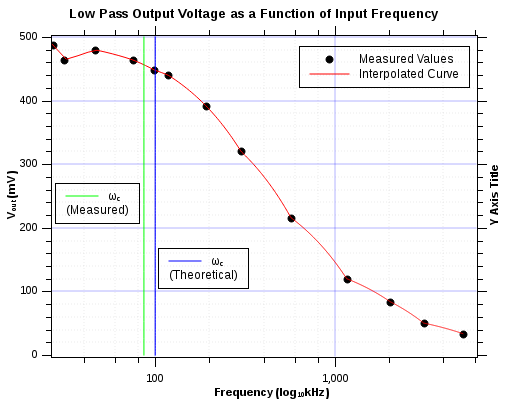
\includegraphics[width=.8\linewidth]{./Graphs/LowPass.png}
			\caption{Plot of Low Pass Filter Output Voltage as a Function of Input Frequency}
			\label{graph:lp_output}
			\end{center}
			\par\end{centering}
		\end{figure}

		The collected measurements were then plotted, using the output voltage as a function of frequency in order to show the overall trend. Figure~\ref{graph:lp_output} shows this graph, where the frequency is on a logarithmic scale, and the two calculated values of $\omega_c$ are plotted for reference. The general trend shows that frequencies higher than $\omega_c$ were attenuated, increasingly so at higher frequencies, and that on average frequencies lower than $\omega_c$ were passed.

		In this case, the output voltage was several orders of magnitude lower than the input voltage, and the condition
		\begin{align*}
			V_{out} = \frac{1}{\sqrt{2}}V_{in}
		\end{align*}
		was not met at any frequencies.

\clearpage

\begin{figure}[H]
	\centering
	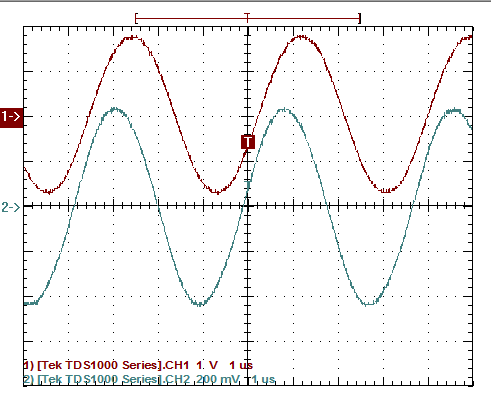
\includegraphics[width=.90\linewidth]{{./Captures/circuit_2_sinewave_265kHz}.PNG}
	\caption{Integrator, Driven by a Low Frequency Sine Wave}
	\label{fig:i1}
\end{figure}
The first three figures depict waves driven at 265 kHz. Here, the input signal is shown above, and the output signal below it. Comparing this to the differentiated sine wave in Figure~\ref{fig:d1} shows that the outputs of the two circuits are nearly identical. However, this behavior is instead exhibited at low frequencies instead of high frequencies. The similarity is consistent with the behavior of sinusoids, for which the derivative and the integral are the same function (within a multiplicative constant).
\vfill
\begin{figure}[H]
	\centering
	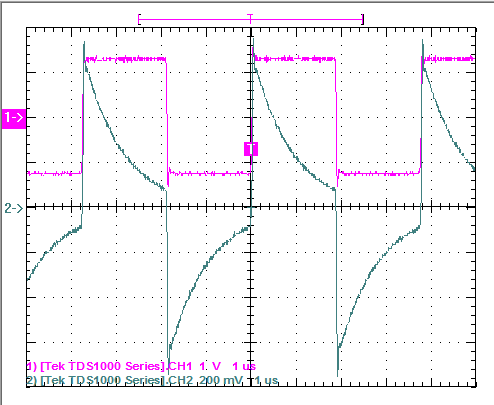
\includegraphics[width=.90\linewidth]{{./Captures/circuit_2_squarewave_265kHz}.PNG}
	\caption{Integrator, Driven by a Low Frequency Square Wave}
	\label{fig:i2}
\end{figure}
The square wave input at 265 kHz shown above exhibits the physical limitations of the integrator. While the output appears to be a straight line in the neighborhood in which the input is constant, increased resolution shows that it is curved slightly. Additionally, regions of abrupt input changes cause amplified output changes, which follows from the fact that a small change in a constant function $k$ is much larger in its antiderivative $kt$.

\break

\begin{figure}[H]
	\centering
	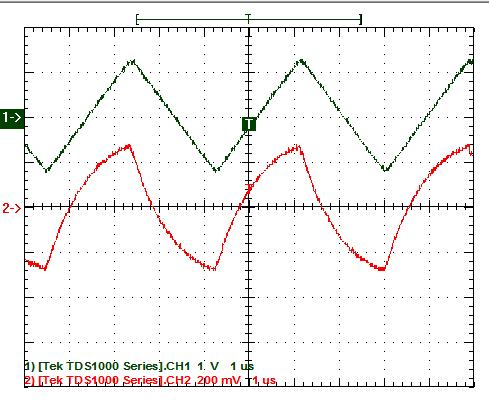
\includegraphics[width=.90\linewidth]{{./Captures/circuit_2_tri_wave_265kHz}.PNG}
	\caption{Integrator, Driven by a Low Frequency Triangle Wave}
	\label{fig:i3}
\end{figure}
The integrator's output given a triangle wave and driven at 256 kHz exhibits similar behavior as the differentiator (Figure~\ref{fig:d3}). The exponential behavior of the capacitor is again seen, but in this case on the order of $\mu$s instead of ns. A key difference is that at the peaks of the triangle wave are preserved -- while the derivative may not be defined at these points, the antiderivative can still be calculated.
\vfill
\begin{figure}[H]
	\centering
	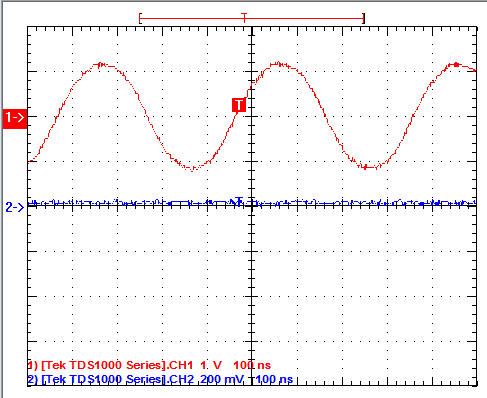
\includegraphics[width=.90\linewidth]{{./Captures/circuit_2_sinewave_2.5MHz}.PNG}
	\caption{Integrator, Driven by a High Frequency Sine Wave}
	\label{fig:i4}
\end{figure}
When driven at 2.5 MHz, the limiting behavior becomes apparent. The output appears sinusoidal, but becomes incredibly in amplitude. This is again consistent with the notion that a capacitor can not change voltage instantaneously, and begins to behave like a wire at high frequencies. This would leads to an $\Delta V_{rms}$ of 0, which the capacitor approaches as the frequency approaches infinity.

\clearpage



	\subsection{High-Pass Filter}
	The measurements and analysis made for the Low-Pass Filter were repeated for this circuit, and the results are summarized in Table~\ref{tb:hp_output} and Figure~\ref{graph:hp_output}.

		\begin{table}[H]
			\caption{High-Pass Filter RMS Output Voltage at Varying Frequencies}
			\label{tb:hp_output}
			\centering
		\begin{tabular}{@{}lll@{}}
		\toprule
		Frequency    & $V_{in}$ (V) & $V_{out}$ (V) \\
		\midrule
		\textit{kHz} &      	&       \\
		27           & 21.2 	& 1.20  \\
		66           & 21.0   	& 2.40  \\
		91           & 21.2 	& 3.04  \\
		138          & 21.0   	& 4.00  \\
		233          & 21.0   	& 5.04  \\
		496          & 21.0   	& 6.08  \\
		674          & 21.0   	& 6.24  \\
		\midrule
		\textit{MHz} &      	&       \\
		1.17         & 21.0   	& 6.40  \\
		1.71         & 21.0   	& 6.48  \\
		2.50         & 20.6 	& 6.48  \\
		3.13         & 20.2 	& 6.32  \\
		4.52         & 20.0   	& 6.08  \\
		5.19         & 19.2 	& 6.00  \\ \bottomrule
		\end{tabular}
		\end{table}

		Inspection of the values in Table~\ref{tb:hp_output} shows that the behavior of the High-Pass Filter is opposite that of the Low-Pass Filter, and that the output voltage is constant at high frequencies and attenuated at low frequencies. In this case, however, the voltage drop is much higher (on the order of volts instead of millivolts) and occurs in the range of 200-400 kHz, a significant deviation from the the theoretical $\omega_c$ of 100 kHz and the measured values of 77.6 kHz. However, it is as the frequency approaches 100 kHz, the output voltage has drops to less than 64\% of its initial value, and maintains the same trend, which is shown more clearly in Figure~\ref{graph:hp_output}.

		\begin{figure}[H]
			\begin{centering}
			\begin{center}
			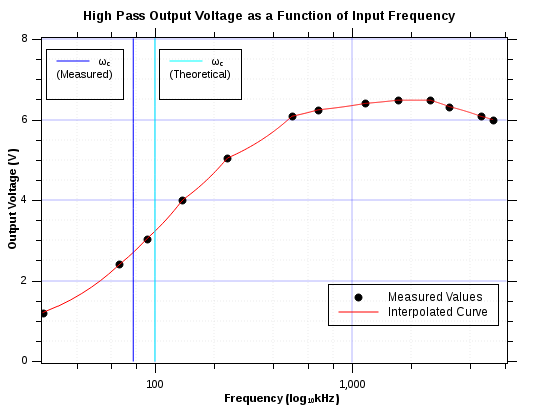
\includegraphics[width=\linewidth]{./Graphs/HighPass.png}
			\caption{Plot of High Pass Filter Output Voltage}
			\label{graph:hp_output}
			\end{center}
			\par\end{centering}
		\end{figure}
		This plot shows the data plotted from Table~\ref{tb:hp_output}, with output voltage as a function of frequency on a logarithmic scale, and the theoretical values of $\omega_c$ are marked respectively. In general, the data shows that signals above $\omega_c$ tend to be passed, while those below are nearly dropped entirely. However, it appears that the attenuation begins at much higher frequencies than $\omega_c$. This may be due to imprecision in measurements or insufficient data. It is also possible that this filter has a range of ``fuzziness'', inside of which the signal may be dropped slightly. If this is the case, building such circuits for applications may require choosing the cutoff frequency much lower than the frequencies chosen to pass through, so as not to inadvertently lose signal information.

	\subsection{Band-Pass Filter}

	\begin{figure}[H]
			\begin{centering}
			\begin{center}
			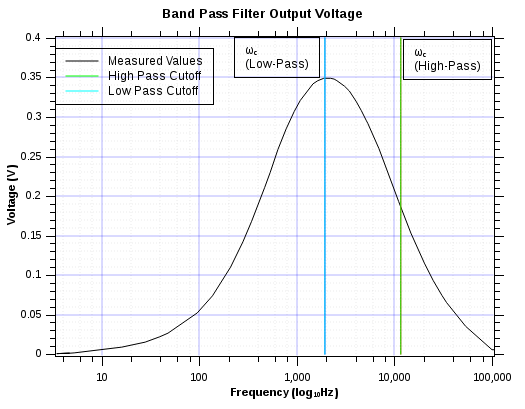
\includegraphics[width=\linewidth]{./Graphs/BandPass.png}
			\caption{Plot of High Pass Filter Output Voltage}
			\label{graph:hp_output}
			\end{center}
			\par\end{centering}
		\end{figure}
		The Band-Pass Filter was constructed as a combination of a High-Pass and a Low-Pass filter in parallel. In order to examine its behavior, a similar analysis to the previous circuits was applied -- multiple output voltage measurements were taken over a range of frequencies. From the measured values, it was found that the cutoff frequencies for each portion were 1.94 kHz and 11.6 kHz, respectively. These values, along with a plot of the measured value, shows that frequencies outside of this range were attenuated, and frequencies inside of this range were passed to the output.


\onecolumn
\appendices{}

\section{Circuit Photographs}
\begin{figure}[H]
			\begin{centering}
			\begin{center}
			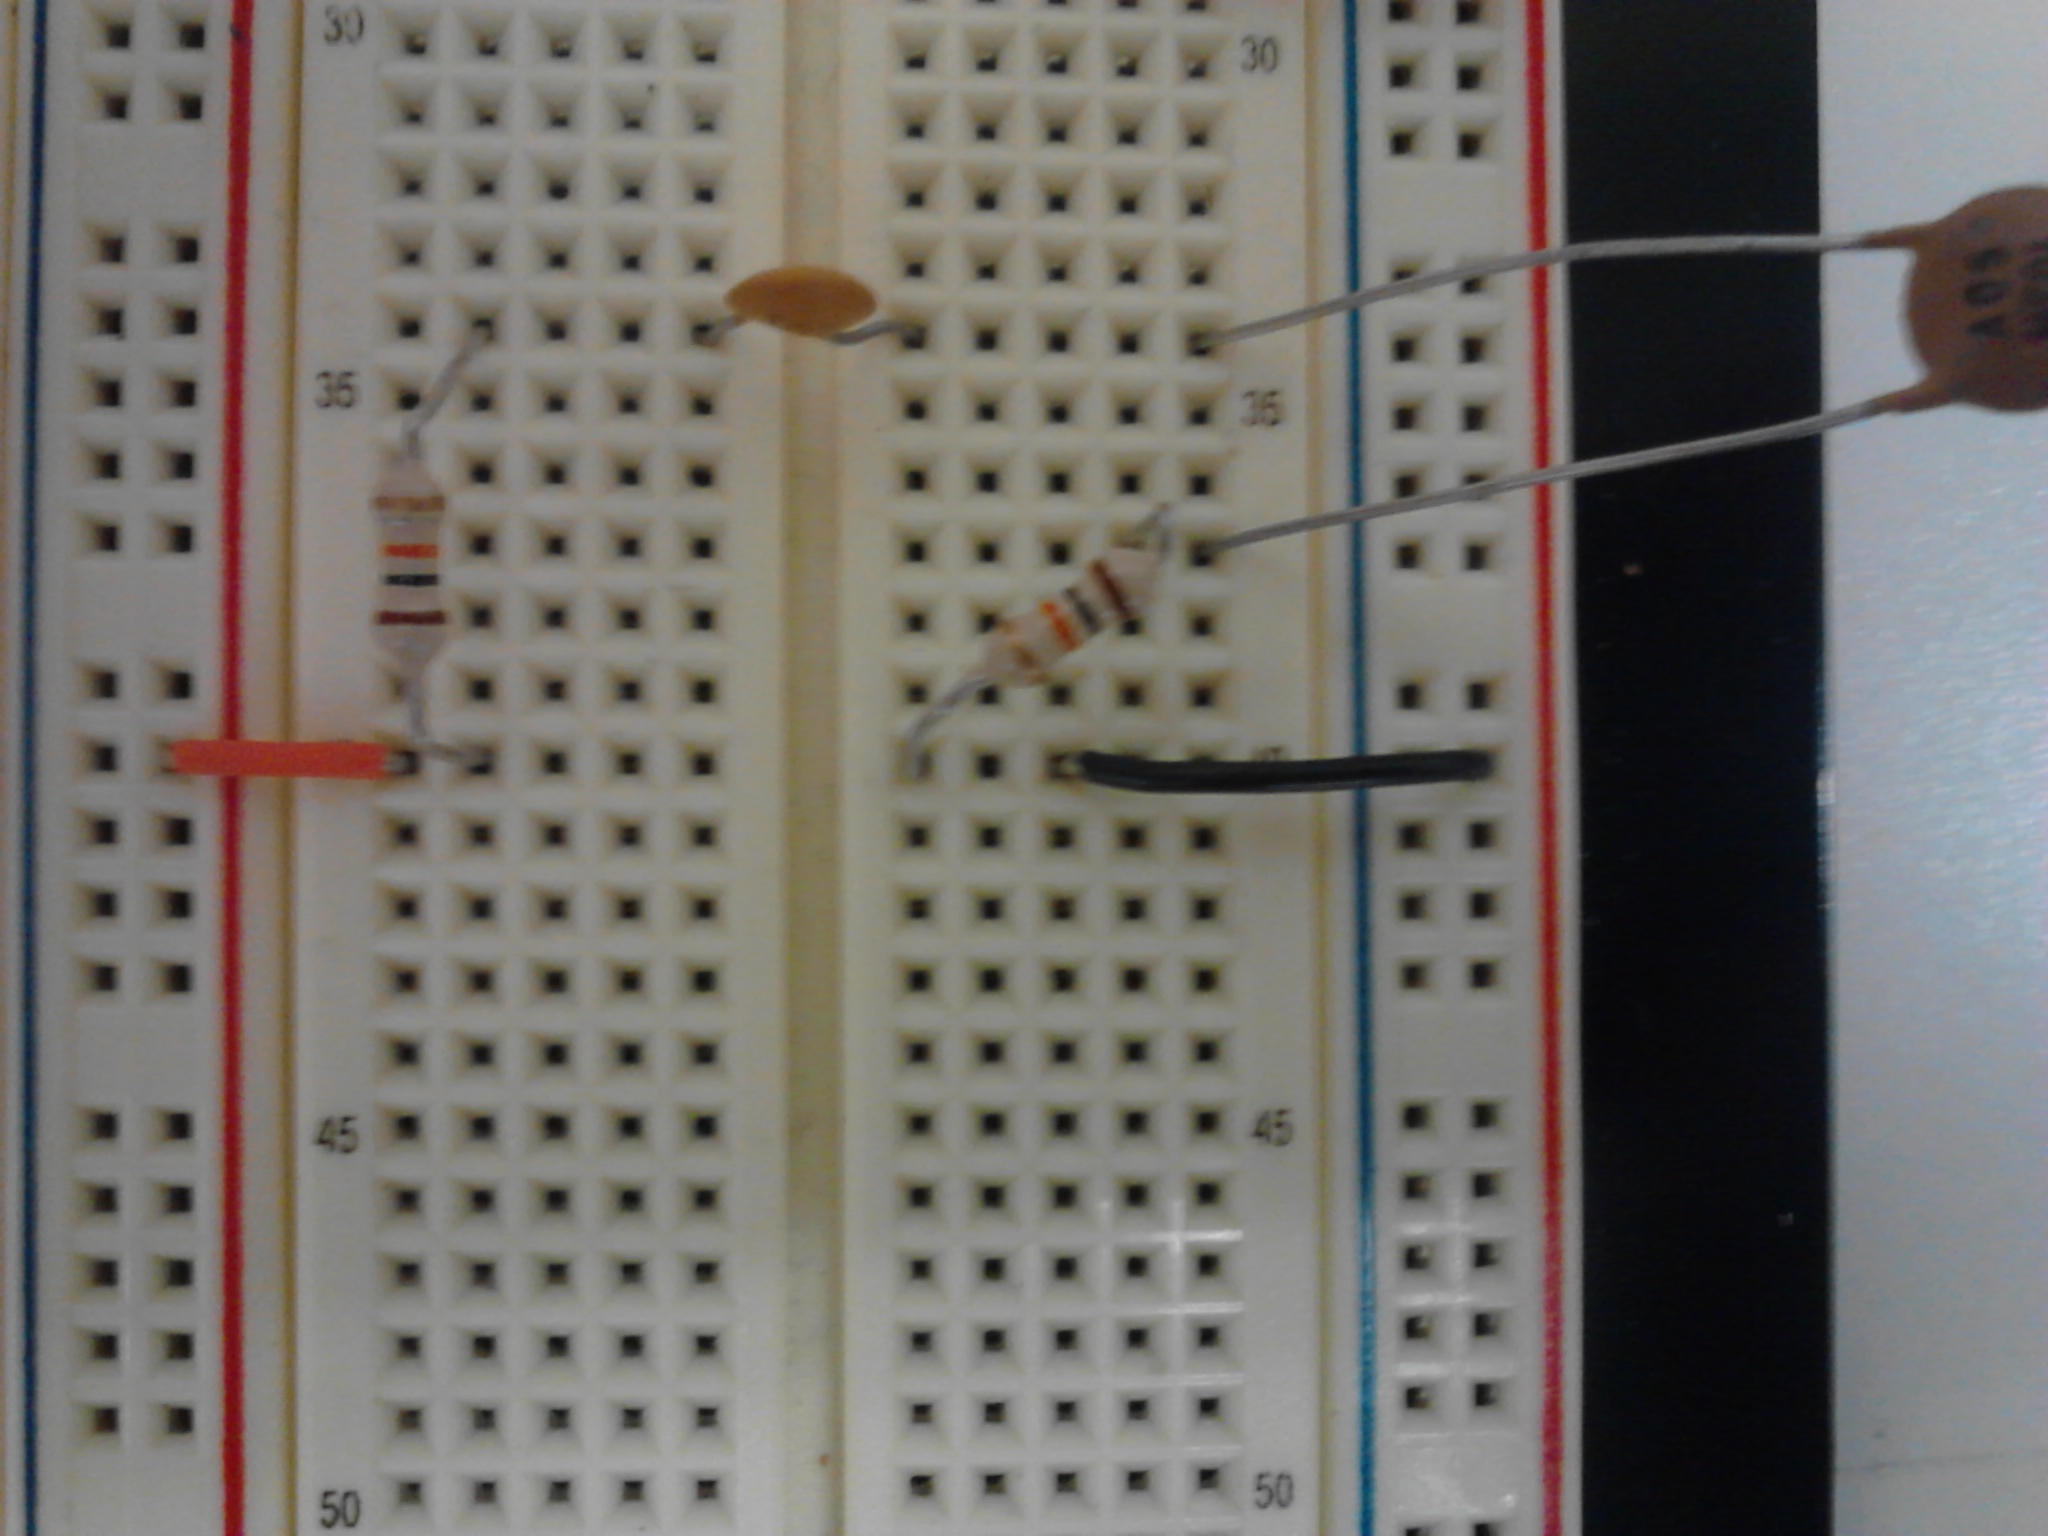
\includegraphics[width=\linewidth]{./bp_photo.png}
			\caption{Photograph of the Band Pass Filter}
			\label{graph:bp_photo}
			\end{center}
			\par\end{centering}
		\end{figure}


%\bibliographystyle{plain}
%\bibliography{physbib}

\begin{thebibliography}{9}
\centering
\bibitem{wiki-differentiator}
	``Differentiator.''
	Wikipedia.
	Wikimedia Foundation, 18 Apr. 2014.
	Web.
	19 Apr. 2014.
\bibitem{wiki-integrator}
	``Passive Integrator Circuit.''
	Wikipedia.
	Wikimedia Foundation, 18 Apr. 2014.
	Web.
	20 Apr. 2014.
\end{thebibliography}

\end{document}